\section{Recurrency}

Adaptive learning in concept drift.
Predictability of events in the data stream.
Sums of independent random variables.
Recurrency is a form of predictability.



\section{Pccf }~\label{sec:pccf}
From~\cite{Maslov2021}.
If change points are expected to reoccur in the input signal, then this prior information can be used to approximate prediction time intervals, or regions of interest (ROI), where changes are most likely to appear in the future.
Once calculated, and if predictions are correct, then this information can further be used to reduce the false alarm rate of the change detection process, and potentially to reduce detection delays too.
FA rate can be decreased just by disregarding detections outside prediction intervals, and the detection delay can be decreased by increasing sensitivity of the detector within prediction intervals.
But, as mentioned, if sensitivity is increased, then probability of FA events will also increase.
Possibility of decreasing detection delays in the presence of prediction interval is a subject of Experiments section.
We describe next how to calculate prediction intervals for reoccurring change points.

To calculate ROIs for recurrent change points we use a prediction confidence change function (Pccf) proposed in our previous work~\cite{MaslovSDM2016}, where it was calculated using convolutions.
Below we calculate Pccf for several commonly used distributions of inter-arrival times values using moment generating functions, what is a more concise way than when using convolutions.
Let's start with definitions.
\begin{definition}
	Change points $t_i^{\text{c}}$ are recurrent if their inter-arrival times $t_{i}^{c} - t_{i-1}^{c}$
	% \begin{equation}\label{eq:recurrence_relation}
	%     \Delta_i = t_{i}^{c} - t_{i-1}^{c}
	% \end{equation}
	are i.i.d.\ from the same probability distribution.
	E.g., $t_{i}^{c} - t_{i-1}^{c} \sim \mathbb{N}(\mu, \sigma)$ if $\sigma$ is small.
\end{definition}
%The recurrence relation for recurrent changes is \begin{equation} x_{n+1} = x_n + \delta_n \end{equation}
Pccf function value at time moment $t_i$ is a probability estimator of recurrent change point to occur at this time moment.
%Recurrent changepoints form a sequence determined by recurrence relation given by Equation~\ref{eq:recurrence_relation}.
% $t_{i}^{\text{CHP}} = t_{i-1}^{\text{CHP}} + \Delta_i$.
Pccf can be represented as a matrix~\ref{eq:pccf_matrix} in which elements at row $k$ and column $i$ are probability estimates for change point $t_k^{\text{c}}$ to appear at time moment $t_i$.
\begin{equation}~\label{eq:pccf_matrix}
	\text{PCCF}_{k,i} \equiv P(t_{k}^{\text{c}} = t_i) % \: \forall \:  k, i \in [1,\dots,N
\end{equation}
When calculating ROIs we are interested in total probability of any changepoint occurring at every time moment within prediction horizon.
Since events $t_k^{\text{c}} = t_i$ are disjoint we need to sum up rows of the matrix $\text{PCCF}_{k,i}$
\begin{equation}~\label{eq:pccf_vector}
	\text{PCCF}_{i \in 1:N} = \sum_{k=1}^{N} P(t_k^{\text{c}} = t_i) \equiv \sum_{k=1}^{N} \text{PCCF}_{k,i}
\end{equation}
Further by Pccf we call the vector given by Equation~\ref{eq:pccf_vector}.

The sum~\ref{eq:pccf_vector} can be calculated using the notion of moment generating function (Mgf).
As an example, let's assume a Gaussian distribution for inter-arrival times, i.e. $t_{i}^{\text{c}} - t_{i-1}^{\text{c}} \sim \mathbb{N}(\mu, \sigma)$,
with $\sigma$ small enough so that every next change can not happen before the previous one.
For example, if $\mu=60$ seconds and standard deviation is $\sigma=5$ seconds then, using Chebyshev's inequality~\ref{eq:chebyshev_ineq}, probability of
$\mathbb{P}(|t_{i}^{\text{c}} - t_{i-1}^{\text{c}}| \geq 60) \leq 0.007$.
\begin{equation}\label{eq:chebyshev_ineq}
	\mathbb{P}(|X-\mu| \geq k \sigma) \leq \frac{1}{k^2} % %\mathbb{P}(|X-\mu| \geq t) \leq \frac{\sigma^2}{t^2}
\end{equation}
By definition, Mgf, or Laplace transform, of random variable $X$ is~\ref{eq:mgf}
%~\footnote{Mgf is $\mathbb{E}(e^{tX})$ while characteristic function is $\mathbb{E}(e^{i t X})$.}
\begin{equation}\label{eq:mgf}
	M_{X}(t) = \mathbb{E}(e^{t X}), \: t \in \mathbb{R}
\end{equation}
Using the property that expected value of the product of two independent random variables is the product of their expected values $\mathbb{E}(X \dot Y)=\mathbb{E}(X)\mathbb{E}(Y)$, Mgf of the sum of independent random variables is a product of individual Mgfs (Equation~\ref{eq:mgf_of_sum}).
\begin{equation}\label{eq:mgf_of_sum}
	M_{X+Y}(t) = \mathbb{E}(e^{t (X+Y)}) = \mathbb{E}(e^{t X}) \mathbb{E} (e^{t Y}) \equiv M_{X}(t) M_{Y}(t)
\end{equation}
For the Gaussian distribution Mgf is $\exp{(\mu t + \frac{\sigma^2 t^2}{2})}$ and therefore
\begin{equation}\label{eq:mgf_gauss}
	M_{X+Y}^{\text{Gaussian}}(t)  = \exp \Big ((\mu_X + \mu_Y) t + \frac{(\sigma_X^2 + \sigma_Y^2) t^2}{2} \Big )
\end{equation}
But~\ref{eq:mgf_gauss} is Mgf of the Gaussian distribution with parameters $\mu=\mu_1+\mu_2$ and $\sigma=\sqrt{\sigma_X^2 + \sigma_Y^2})$.
Therefore if probability distribution of the first change point is $t_1^{\text{c}} \sim \mathbb{N}(\mu, \sigma)$ then $t_2^{\text{c}} \sim \mathbb{N}(2\mu, \sigma \sqrt{2})$, etc.
And Pccf is a sum~\ref{eq:pccf_gaussian}
\begin{equation}\label{eq:pccf_gaussian}
	\text{PCCF}^{\text{Gaussian}} \equiv \sum_{k=1}^N \mathbb{N}(k \mu, \sqrt{k} \sigma)
\end{equation}

Using the same logic it is straightforward to calculate Pccfs for Exponential and Gamma distributions (Table~\ref{table:pccfs}).
\begin{table}[!htb] \caption{Pdf's for distributions of inter-arrival times.}\label{table:pccfs}
	\begin{center}
		\begin{tabular}{|l|l|c|c|}
			\hline
			Distribution & Mgf & PDF of the $k$-th event & PCCF  \\[5pt]
			\hline
			Gaussian & $\exp{ (\mu t + \frac{\sigma^2 t^2}{2}) }$ & $\mathcal{N}(k \mu, \sqrt{k} \sigma)$ & $\sum_{k=1}^N \mathcal{N}(k \mu, \sqrt{k} \sigma)$ \\
			Gamma $\Gamma(\alpha, \lambda)$ & $\Big ( \frac{1}{1- \lambda t} \Big )^{\alpha}$ & $\Gamma(k \alpha, \lambda)$ & $\sum_{k=1}^N \Gamma(k \alpha, \lambda)$\\
			Exponential & $\frac{\lambda}{\lambda - t}$ & $\Gamma(k, \lambda)$ & $\sum_{k=1}^N \Gamma(k, \lambda)$\\
			\hline
		\end{tabular}
	\end{center}
\end{table}
Figure~\ref{fig:pccf_example} depicts Gaussian Pccf.
Prediction intervals (ROI) can be calculated by applying a threshold value for Pccf and then ROIs will be determined by time moments when Pccf exceeds this threshold.
In this way we would take into account uncertainty in the predictions for $k$-th change points which will increase as $\sqrt{k} \sigma$ (Equation~\ref{eq:pccf_gaussian}).
Another way is to use the property that Pccf extremums are equally spaced (Equation~\ref{eq:rois})~\cite{MaslovSDM2016} by time intervals $\mu$.
After estimating $\mu$ between changes and choosing the number of change points $k$ to predict and ROIs width prediction interval are determined by Equation~\ref{eq:rois}.
\begin{equation}\label{eq:rois}
	\text{ROI}s = (\mu \pm \text{ROI}_{\text{Width}}, 2 \mu \pm \text{ROI}_{\text{Width}}, \dots , k \mu \pm \text{ROI}_{\text{Width}}).
\end{equation}
\begin{figure}[!htb]
	\centering
	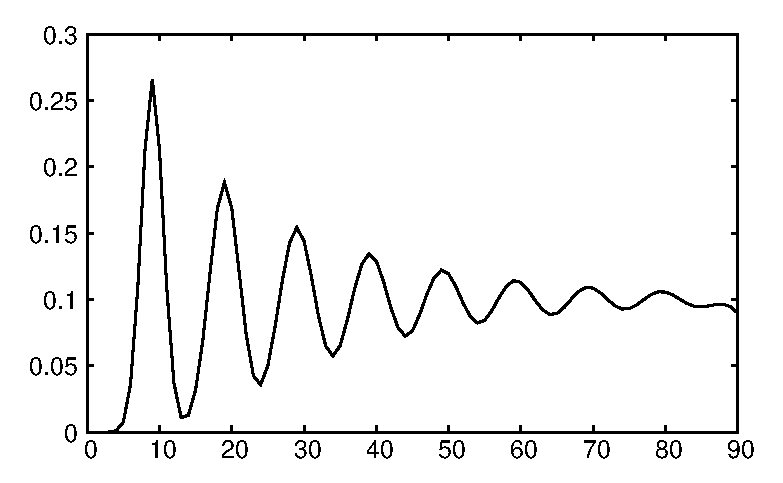
\includegraphics[width=0.7\textwidth]{images/example_pccf.eps}
	\caption{Pccf example}\label{fig:pccf_example}
\end{figure}

